\documentclass[a4paper,12pt]{article} % добавить leqno в [] для нумерации слева
\usepackage[a4paper,top=1.3cm,bottom=2cm,left=1.5cm,right=1.5cm,marginparwidth=0.75cm]{geometry}
%%% Работа с русским языком
\usepackage{cmap}					% поиск в PDF
\usepackage[warn]{mathtext} 		% русские буквы в фомулах
\usepackage[T2A]{fontenc}			% кодировка
\usepackage[utf8]{inputenc}			% кодировка исходного текста
\usepackage[english,russian]{babel}	% локализация и переносы
\usepackage{physics}
\usepackage{multirow}
\usepackage{siunitx}

%%% Нормальное размещение таблиц (писать [H] в окружении таблицы)
\usepackage{float}
\restylefloat{table}

\usepackage{graphicx}

\usepackage{caption}
\usepackage{subcaption}

\usepackage{wrapfig}
\usepackage{tabularx}

\usepackage{hyperref}
\usepackage[rgb]{xcolor}
\hypersetup{
	colorlinks=true,urlcolor=blue
}

%%% Дополнительная работа с математикой
\usepackage{amsmath,amsfonts,amssymb,amsthm,mathtools} % AMS
\usepackage{icomma} % "Умная" запятая: $0,2$ --- число, $0, 2$ --- перечисление

%% Номера формул
%\mathtoolsset{showonlyrefs=true} % Показывать номера только у тех формул, на которые есть \eqref{} в тексте.

%% Шрифты
\usepackage{euscript}	 % Шрифт Евклид
\usepackage{mathrsfs} % Красивый матшрифт
\usepackage{pgfplots}
\pgfplotsset{compat=1.9}

%% Свои команды
\DeclareMathOperator{\sgn}{\mathop{sgn}}

%% Не нумеровать секциии
\setcounter{secnumdepth}{0}

%% Перенос знаков в формулах (по Львовскому)
\newcommand*{\hm}[1]{#1\nobreak\discretionary{}
	{\hbox{$\mathsurround=0pt #1$}}{}}

\date{\today}

\begin{document}

\begin{titlepage}
	\begin{center}
		{\large МОСКОВСКИЙ ФИЗИКО-ТЕХНИЧЕСКИЙ ИНСТИТУТ (НАЦИОНАЛЬНЫЙ ИССЛЕДОВАТЕЛЬСКИЙ УНИВЕРСИТЕТ)}
	\end{center}
	\begin{center}
		{\large Физтех-школа прикладной математики и информатики}
	\end{center}
	
	
	\vspace{4.5cm}
	{\huge
		\begin{center}
			{\bf Отчёт о выполнении лабораторной работы 4.2}\\
			Исследование энергетического спектра $\beta$-частиц и определение их максимальной энергии при помощи магнитного спектрометра
		\end{center}
	}
	\vspace{1cm}
	\begin{center}
		{\large Соболевский Федор Александрович \\
			\vspace{0.2cm}
			Б05-111}
	\end{center}
	\vspace{8cm}
	\begin{center}
		  Ноябрь 2023
	\end{center}
\end{titlepage}

\section{Теоретические положения}

\textbf{Бета-распад}~--  это самопроизвольное превращение ядер, при котором их массовое число не изменяется, а заряд изменяется на единицу. В данной работе мы будем иметь дело с электронным распадом:
\begin{equation}
    _{Z}^{A}X \rightarrow _{Z+1}^{A}X + e^{-} + \widetilde{\nu}.
\end{equation}
Освобождающаяся в результате распада энергия делится между исходным ядром, электроном и нейтрино. При этом доля энергии, уносимая ядром крайне мала, так что вся энергия делится между нейтрино и электроном. Поэтому электроны могут иметь любую энергию от нулевой до некоторой максимальной энергии, высвобождаемой при распаде.
		
Вероятность $d\omega$ того, что электрон вылетит с импульсом $d^3\mathbf{p}$, а нейтрино с импульсом $d^3\mathbf{k}$ равна произведению этих дифференциалов, но мы должны учесть также закон сохранения энергии.
\begin{equation}
    E_e - E - ck = 0,
\end{equation}
где $E_e$~-- максимальная энергия электрона, $E$~-- кинетическая энергия электрона:
\begin{equation}
    E = c\sqrt{p^2 + m^2c^2} -mc^2,
\end{equation}
а через $ck$ обозначена энергия антинейтрино с импульсом $k$. Таким образом, вероятность $d\omega$ принимает вид:
\begin{equation}
    d\omega = D\delta(E_e-E-ck)d^3\mathbf{p}d^3\mathbf{k} = D\delta(E_e-E-ck)p^2d pk^2d kd\Omega_ed\Omega_{\widetilde{\nu}},
\end{equation}
где $D$~-- некоторый коэффициент пропорциональности, $\delta$~-- дельта-функция, $d\Omega_e$ и $d\Omega_{\widetilde{\nu}}$~-- элементы телесных углов направлений вылета электрона и нейтрино. В случае рассматриваемых нами разрешенных фермиевских типов распадов $D$ можно считать с хорошей точностью константой. В этом случае можно проинтегрировать по всем углам и по абсолютному значению импульса нейтрино; $\delta$-функция исчезнет, а $ck$ всюду заменится на $E_e-E$. После умножения на полное число распадов проинтегрированное выражение приобретает смысл числа электронов $dN$, вылетающих из ядра с импульсом, абсолютная величина которого лежит между $p$ и $p +dp$:
\begin{equation}
    \dif N = \frac{16\pi^2N_0}{c^2} D p^2\left(E_e-E\right)^2\dif p
\end{equation}
Чтобы получить распределение электронов по энергиям, необходимо перейти от $dp$ к $dE$. Получаем выражение:
\begin{equation}
    \frac{dN}{dE} = N_0B\sqrt{E(E+2mc^2)}(E_e - E)^2(E+mc^2),
\end{equation}
где $B = (16\pi^2/c^4)D$. В нерелятивистском случае выражение упрощается и принимает вид:
\begin{equation}
    \frac{d N}{d E} \simeq \sqrt{E}(E_e - E)^2
\end{equation}
Данное выражение определяет форму спектра $\beta$-распада. Дочерние ядра, возникающие в результате $\beta$-распада, нередко оказываются возбуждёнными. Возбуждённые ядра отдают свою энергию либо излучая гамма-квант, либо передавая избыток энергии одному из электронов с внутренних оболочек атома (обычно $K$ или $L$). Последние электроны имеют строго определённую энергию и называются \textit{конверсионными}. Ширина монохроматической линии, соответствующая конверсионным электронам, определяет разрешающую силу спектрометра (см. рис. \ref{fig:spectre}).
\begin{figure}[h]
    \centering
    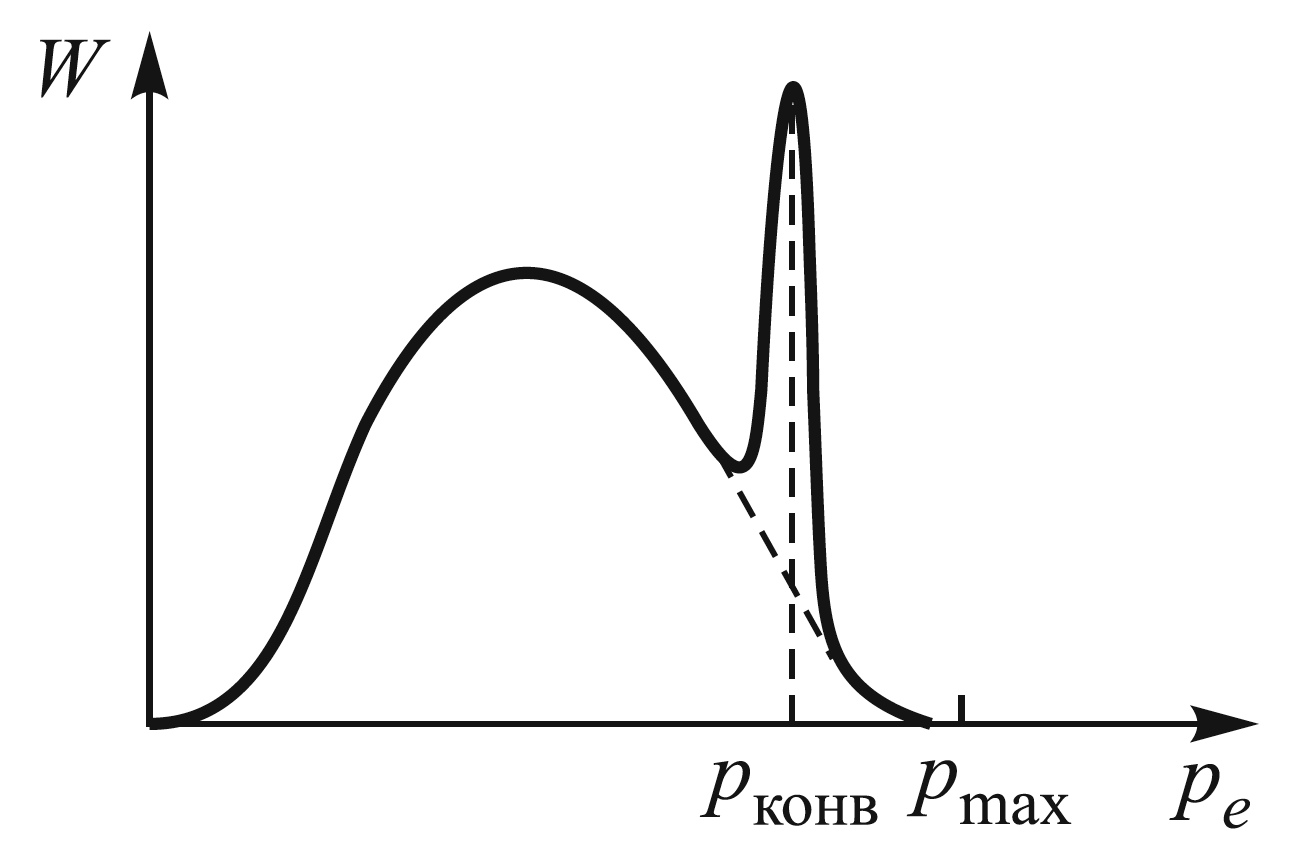
\includegraphics[width=0.5\textwidth]{spectre.png}
    \caption{Вид энергетического спектра $\beta$-излучения}
    \label{fig:spectre}
\end{figure}

\section{Экспериментальная установка}
Энергию частиц определяют с помощью $\beta$-спектрометров. В работе используется магнитный спектрометр с <<короткой>> линзой, сцинтиллятором и ФЭУ (см. рис. \ref{ris:experimoriginal}, \ref{ris:experimcoded}). Как показывает расчет, для заряженных частиц тонкая катушка эквивалентна линзе:
\begin{equation}
    \frac{1}{f} \simeq \frac{I^2}{p_e^2}
\end{equation}
При заданной силе тока на входное окно счетчика собираются электроны с определенным импульсом. Импульс сфокусированных электронов пропорционален силе тока:
\begin{equation}\label{proportion}
    p_e = kI.
\end{equation}
Коэффициент пропорциональности $k$ обычно определяется по какой-либо известной конверсионной линии.
\begin{figure}[h]
\begin{center}
\begin{minipage}[h]{0.48\linewidth}
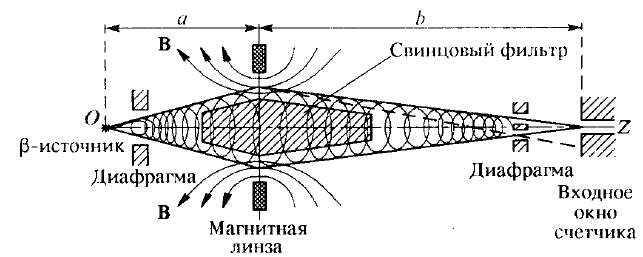
\includegraphics[width=1\linewidth]{lens.PNG}
\caption{Схема $\beta$-спектрометра с короткой магнитной линзой} %% подпись к рисунку
\label{ris:experimoriginal}
\end{minipage}
\hfill 
\begin{minipage}[h]{0.48\linewidth}
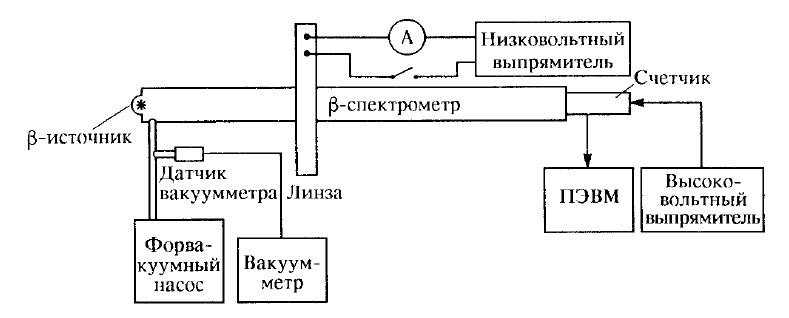
\includegraphics[width=1\linewidth]{setup.PNG}
\caption{Блок-схема установки для изучения $\beta$-спектра}
\label{ris:experimcoded}
\end{minipage}
\end{center}
\end{figure}

\section{Результаты измерений и обработка экспериментальных данных}
\subsection{Определение фона}
Измерение фона было проведено 5 раз. Результаты и погрешности их определения представлены в таблице \ref{tab:background}.
\begin{table}[h]
    \centering
    \begin{tabular}{|c|c|c|c|c|c|} \hline
        Номер измерения & 1 & 2 & 3 & 4 & 5 \\ \hline
        $N_\text{ф},\text{ с}^{-1}$ & 0,6797 & 0,8196 & 0,5197 & 0,6197 & 0,6397 \\ \hline
        $\Delta,\text{ с}^{-1}$ & 0,117 & 0,128 & 0,102 & 0,111 & 0,113 \\ \hline
    \end{tabular}
    \caption{Результаты измерения фона}
    \label{tab:background}
\end{table}

Будем использовать усреднённое значение:
\begin{equation*}
    \overline{N_\text{ф}} = 0,656 \text{ с}^{-1},\quad \sigma = \frac{1}{5 - 1}\sqrt{\sum\limits_{i=1}^5 (N_{\text{ф}_i} - \overline{N_\text{ф}})^2} = 0,054 \text{ с}^{-1},\quad \sigma_\text{полн} = \sqrt{\sigma^2 + \overline{\Delta}^2} = 0,123\text{ с}^{-1}.
\end{equation*}

\subsection{Измерение спектра $\beta$-частиц}
Определим коэффициент пропорциональности в формуле \eqref{proportion} по току, соответствующему пику конверсии $T_\text{к} = 0,624$ МэВ:
\[
    I_\text{конв} = 4,25\text{ А},\quad k = \frac{T_\text{к}}{I_\text{к}c} = 0,489\cdot 10^{-3} \frac{\text{эВ}}{c\cdot\text{А}},\quad \sigma_k = k\frac{\sigma_I}{I} = 0,005\cdot 10^{-3} \frac{\text{эВ}}{c\cdot\text{А}}.
\]

По этому коэффициенту теперь можно определить $p_e$ и $T$ $\beta$-частиц, зная ток в установке. Результаты измерения спектра представлены в таблице \ref{tab:graph_data}. По этим данным построены графики зависимости частоты частиц от тока (рис. \ref{fig:curr_plot}) и импульса/энергии (рис. \ref{fig:imp_plot}).

\begin{figure}[h]
\begin{center}
\begin{minipage}[h]{0.49\linewidth}
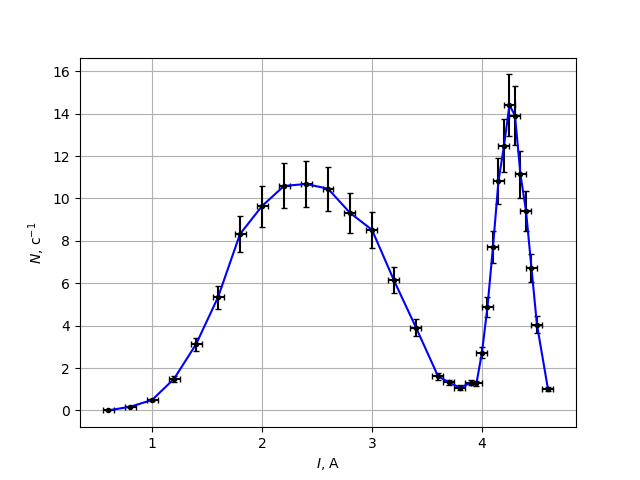
\includegraphics[width=1\linewidth]{curr_plot.png}
    \caption{Зависимость частоты $\beta$-частиц от тока в линзе}
    \label{fig:curr_plot}
\end{minipage}
\hfill 
\begin{minipage}[h]{0.49\linewidth}
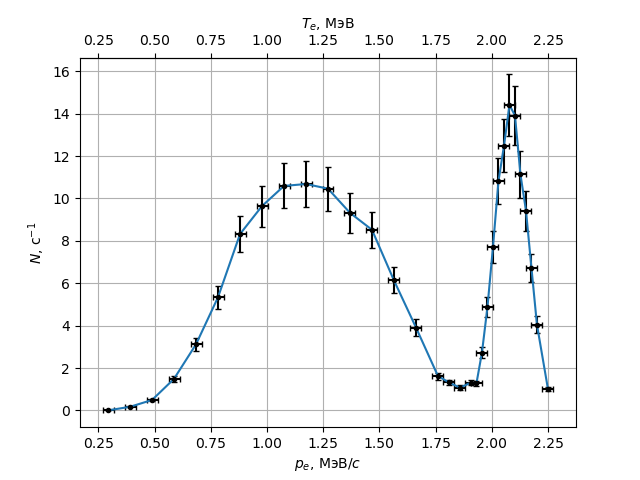
\includegraphics[width=1\linewidth]{imp_plot.png}
    \caption{Импульсный и энергетический спектр $\beta$-частиц}
    \label{fig:imp_plot}
\end{minipage}
\end{center}
\end{figure}

\subsection{Расчет максимальной энергии электронов}
Чтобы точнее определить максимуальную энергию электрона $T_\text{max}$, используем график Ферми. По осям ординат и абсцисс отложим соответственно 
$\sqrt{N(p_e)} / p_e^{3/2} \sim T_\text{max} - T$. Выделяем линейную часть графика, соответствующую части электронов, которые не замедлены кулоновским притяжением, но еще не попадают под пик. Установив ее пересечение с осью абсцисс, получаем значение 
\[
T_\text{max} \approx (0,58 \pm 0,02)~ \text{МэВ},
\]
где погрешность рассчитана по формуле:
\begin{equation*}
\sigma(k) = \sqrt{\frac {1}{N - 1} \left(\frac{D_{yy}}{D_{xx}} - k^2 \right)}, ~~~ \sigma_b = \sigma_k  \sqrt{\langle x^2 \rangle}.
\end{equation*}
Это хорошо сходится с табличным значением примерно в $600 \text{КэВ}$.

\begin{figure}[h]
    \centering
    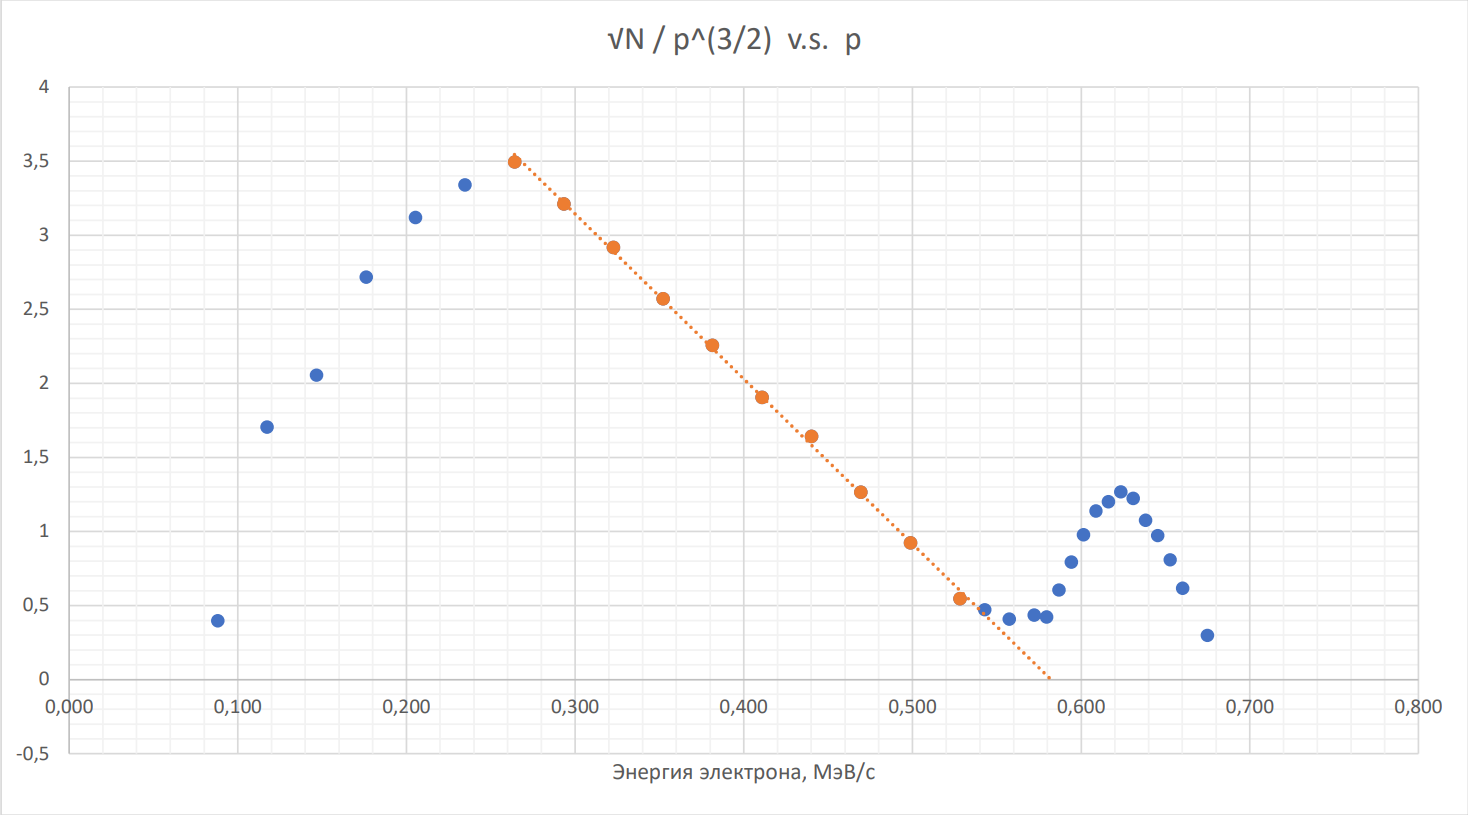
\includegraphics[width=1\textwidth]{Plot2.png}
    \caption{График для определения $T_\text{max}$}
    \label{fig:plot2}
\end{figure}

\section{Вывод}
Нам удалось довольно точно измерить энергетический спектр $\beta$-частиц. Теоретические предположения о пике конверсии и расположении максимума энергий подтвердились на практике. Полученное значение максимума близко к табличному.

\newpage
\section{Приложение}
\begin{table}[h]
    \centering
    \begin{tabular}{|c|c|c|c|c|} \hline
        $I$, A & $p_e$, МэВ/$c$ & $T$, МэВ & $N_\text{полн}$, 1/с & $N$, 1/с \\ \hline
        0.6 & 0.088 & 0.088 & 0.66 & 0.004 \\ \hline
        0.8 & 0.117 & 0.117 & 0.83 & 0.174 \\ \hline
        1 & 0.147 & 0.147 & 1.15 & 0.494 \\ \hline
        1.2 & 0.176 & 0.176 & 2.149 & 1.493 \\ \hline
        1.4 & 0.205 & 0.205 & 3.779 & 3.123 \\ \hline
        1.6 & 0.235 & 0.235 & 5.998 & 5.342 \\ \hline
        1.8 & 0.264 & 0.264 & 8.977 & 8.321 \\ \hline
        2 & 0.293 & 0.293 & 10.297 & 9.641 \\ \hline
        2.2 & 0.323 & 0.323 & 11.247 & 10.591 \\ \hline
        2.4 & 1.174 & 0.352 & 11.337 & 10.681 \\ \hline
        2.6 & 1.271 & 0.381 & 11.117 & 10.461 \\ \hline
        2.8 & 1.369 & 0.411 & 9.977 & 9.321 \\ \hline
        3 & 1.467 & 0.440 & 9.177 & 8.521 \\ \hline
        3.2 & 1.565 & 0.469 & 6.788 & 6.132 \\ \hline
        3.4 & 1.663 & 0.499 & 4.569 & 3.913 \\ \hline
        3.6 & 1.760 & 0.528 & 2.279 & 1.623 \\ \hline
        3.7 & 1.809 & 0.543 & 1.979 & 1.323 \\ \hline
        3.8 & 1.858 & 0.557 & 1.729 & 1.073 \\ \hline
        3.9 & 1.907 & 0.572 & 1.969 & 1.313 \\ \hline
        3.95 & 1.932 & 0.579 & 1.939 & 1.283 \\ \hline
        4 & 1.956 & 0.587 & 3.389 & 2.733 \\ \hline
        4.05 & 1.980 & 0.594 & 5.538 & 4.882 \\ \hline
        4.1 & 2.005 & 0.601 & 8.368 & 7.712 \\ \hline
        4.15 & 2.029 & 0.609 & 11.467 & 10.811 \\ \hline
        4.2 & 2.054 & 0.616 & 13.136 & 12.48 \\ \hline
        4.25 & 2.078 & 0.623 & 15.066 & 14.41 \\ \hline
        4.3 & 2.103 & 0.631 & 14.566 & 13.91 \\ \hline
        4.35 & 2.127 & 0.638 & 11.787 & 11.131 \\ \hline
        4.4 & 2.152 & 0.645 & 10.087 & 9.431 \\ \hline
        4.45 & 2.176 & 0.653 & 7.378 & 6.722 \\ \hline
        4.5 & 2.201 & 0.660 & 4.699 & 4.043 \\ \hline
        4.6 & 2.249 & 0.675 & 1.67 & 1.014 \\ \hline
    \end{tabular}
    \caption{Результаты измерения спектра $\beta$-частиц}
    \label{tab:graph_data}
\end{table}

\end{document}
